% ======== 学位論文 (ver1.2.1) ========= %
\RequirePackage{plautopatch}
\RequirePackage[l2tabu, orthodox]{nag}           % 古いものを一掃
% \documentclass[luatex, report, a4paper, 12pt, openany, twoside]{jlreq}  % pLaTeXと揃える場合
\documentclass[luatex, a4paper, 12pt, openany, twoside]{ltjsreport}
% =======  プリアンブル ======== %
% \usepackage{luatexja}                            % LuaTeX-ja
% \usepackage{luatexja-fontspec}                   % LuaTeX-jaでのフォント変更
% \usepackage[ipaex]{luatexja-preset}              % LuaTeX-jaでのフォント変更
\usepackage{graphicx}                            % グラフ描画
\usepackage{amsmath, amssymb}                    % 数式全般
\usepackage{xcolor}                              % 色を付ける
\usepackage{url}                                 % URL
\usepackage{multicol, multirow,booktabs}         % 表作成
\usepackage[luatex,pdfencoding=auto]{hyperref}   % ハイパーリンク
\usepackage{titleps}                             % ノンブル・柱の変更
\usepackage{here}                                % 図の位置の矯正←論文での図はページ上・下に入れるのが普通なので,使う際は注意
\usepackage[section]{placeins}                   % \section毎に図を調整
\usepackage[margin=25truemm]{geometry}           % 余白設定(2023年度 Wordのテンプレートに準拠)
% \usepackage{cite}                                % (↓があるときはコメントアウト)参考文献をBibTeXでIEEEスタイルにする
\usepackage[%
  bibstyle=ieee,
  citestyle=numeric-comp,
  sorting=none,
  doi=false,
  eprint=false,
  url=true%
]{biblatex}                                      % (↑があるときはコメントアウト)参考文献をBibLaTeXでIEEEスタイルにする
% ======== bibLaTeXのファイルとオプション設定 ============ %
\addbibresource{references.bib} % bibファイルを拡張子つきで書く
% ======== ハイパーリンクの設定 by hyperref ========= %
\hypersetup{
  setpagesize=false,
  bookmarks=true,
  bookmarksnumbered=true,
  bookmarkstype=toc,
  colorlinks=true,
  urlcolor=black,
  linkcolor=black,
  citecolor=black
}
% ======== jlreqの各種設定 ========= %
% % 図・表のキャプションの見た目変更
% \jlreqsetup{
%   caption_font=\normalsize,       % captionのフォント設定
%   caption_label_font=\normalsize  % captionのラベルフォント設定
% }
% ↓標準のスタイルの変更例
% \ModifyHeading{chapter}{font=\huge\gtfamily\bfseries}
% \ModifyHeading{section}{font=\Large\gtfamily\bfseries}
% \ModifyHeading{subsection}{font=\large\gtfamily\bfseries}
% \ModifyHeading{subsubsection}{font=\normalsize\gtfamily\bfseries}
% ======== フォント設定 by luatexja-fontspec ========= %
% \setmainfont[Ligatures={Rare,TeX}]{Times New Roman}
% \setmainjfont[BoldFont=Yu Gothic]{Yu Mincho}
% =======  ノンブル、柱の設定 ======== %
% == 目次での設定
% ヘッダーに全ての情報を載せる
\newpagestyle{headtypeTofCstyle}{
  \headrule
  \sethead[\scalebox{1.0}{\textbf{\thepage}}][][]
      {}{}{\scalebox{1.0}{\textbf{\thepage}}}
}
% == 本文での設定
% ヘッダーに全ての情報を載せる
\newpagestyle{headtypestyle}{
  \headrule
  \sethead[\scalebox{1.0}{\textbf{\thepage}}][][第\thechapter 章 \chaptertitle]
      {\thesection\quad\sectiontitle}{}{\scalebox{1.0}{\textbf{\thepage}}}
}
% == 参考文献・での設定
% ヘッダーに全ての情報を載せる
\newpagestyle{headtypestylePlain}{
  \headrule
  \sethead[\scalebox{1.0}{\textbf{\thepage}}][][\chaptertitle]
      {}{}{\scalebox{1.0}{\textbf{\thepage}}}
}
% == 付録での設定
% ヘッダーに全ての情報を載せる
\newpagestyle{headtypestyleAp}{
  \headrule
  \sethead[\scalebox{1.0}{\textbf{\thepage}}][][付録\thechapter \chaptertitle]
      {\thesection\quad\sectiontitle}{}{\scalebox{1.0}{\textbf{\thepage}}}
}
% =======  newcommandの使用例 ======== %
\newcommand{\img}{\mathrm{i}}         % 虚数単位
\newcommand{\e}{\mathrm{e}}           % Napier数
% =======  学位論文の報告者の情報 ======== %
% -- 学位の確認 -- %
\newcommand{\thesis}{修士論文}
\newcommand{\dept}{高知工科大学大学院工学研究科 \\ 基盤工学専攻○○○○工学コース}

% -- 報告者の情報 -- %
\renewcommand{\title}{タイトル(和文)}
\newcommand{\Etitle}{タイトル(英文)}
\newcommand{\studentID}{1XXXXXX}
\renewcommand{\author}{報告者の氏名}
\newcommand{\advisor}{指導教員の氏名と職階}
\renewcommand{\date}{\today}
% -- 表紙の空行による幅 [ \vskip -(2つのタイトルの行数-2)x20pt ] -- %
\newcommand{\adjspace}{\vskip -0pt}  % タイトルが複数行なら調節のために行間を減らす

% =======  表紙・本文のスタート ======== %
\begin{document}

% === 表紙 === %
\include{cover}

% === 目次 === %
\setcounter{page}{0}\pagenumbering{roman}\pagestyle{headtypeTofCstyle}
\tableofcontents
% \listoffigures
% \listoftables

% === 表目次のページ番号がローマ数字にならないバグの回避 === %
\newpage
\clearpage

% === 各種設定 === %
\graphicspath{{./figures/}} % figuresをデフォルトのフォルダにする
% main matterのノンブル・柱の設定
\setcounter{page}{0}\pagenumbering{arabic}
\pagestyle{headtypestyle}  % ノンブル・柱の設定
% ========================= 本文開始 =================================== %

% == 本文
\include{chapter1}
\include{chapter2}

% == 謝辞
\pagestyle{headtypestylePlain} % ノンブル・柱の設定
\addcontentsline{toc}{chapter}{謝辞}
\include{acknowledgement}

% == 参考文献
\pagestyle{headtypestylePlain} % ノンブル・柱の設定
\addcontentsline{toc}{chapter}{参考文献}
\printbibliography[title={参考文献}]  % 参考文献を表示 (biblatex)
% \bibliographystyle{jIEEEtran}  % 参考文献を表示 (bibtex, jIEEEtran.bstを使う場合)
% \bibliography{references}      % 参考文献を表示 (bibtex, .bibは省略)

% == ヘッダー・フッターのバグ回避
\newpage
\clearpage

% == 付録
\appendix  % 付録
\pagestyle{headtypestyleAp}  % ノンブル・柱の設定
\include{appendixA}
\include{appendixB}
\chapter{\LaTeX の環境導入について}
ここまでテンプレートの説明をしてきたが,
まだTeXの環境構築が出来ていないユーザーのために
環境構築の手順を説明する.
作業手順は以下の通りである.
\begin{enumerate}
  \item TeX Liveの導入
  \item VSCodeの導入
  % \item latexmkrcの設定
  \item GitHubの活用
\end{enumerate}
基本的には\cite{Tex_bilud}を参考としている。

\section{TeXLiveの導入}
ここからインストーラーをダウンロードする。
\url{https://www.tug.org/texlive/acquire-netinstall.html}

ページ上のリンク install-tl-windows.exe 
をクリックしてexeファイルをダウンロードする.
install-tl-windows.exeというexeファイルがダウンロードされるので,
実行する.
このとき、セキュリティエラーが出ると思うが無視して実行する.
実行後,図\ref{fig:install_deisplay_1}図\ref{fig:install_deisplay_2}図\ref{fig:install_deisplay_3}までくれば,
インストーラ画面が立ち上がる(\ref{fig:tex_installer}).
\begin{figure}[H]
    \centering
    \includegraphics[keepaspectratio, width=0.5\linewidth]{Install_deisplay_1.png}
    \caption{インストール画面1.}
    \label{fig:install_deisplay_1}
\end{figure}

\begin{figure}[H]
  \centering
  \includegraphics[keepaspectratio, width=0.5\linewidth]{Istall_deisplay_2.png}
  \caption{インストール画面2.}
  \label{fig:install_deisplay_2}
\end{figure}

\begin{figure}[H]
  \centering
  \includegraphics[keepaspectratio, width=0.5\linewidth]{Install_deisplay_3.png}
  \caption{インストール画面3.}
  \label{fig:install_deisplay_3}
\end{figure}

\begin{figure}[H]
  \centering
  \includegraphics[keepaspectratio, width=0.5\linewidth]{TeX_installer.png}
  \caption{インストーラ画面}
  \label{fig:tex_installer}
\end{figure}

次に「高度な設定」を選択する。
図\ref{fig:installer_setting}が表示される.
ここでは、「ディレクション」,「選択するもの」,「オプション」
の設定を変更できる.
「選択するもの」(図\ref{fig:scheme})
でパッケージを変更する.

\begin{figure}[H]
  \centering
  \includegraphics[keepaspectratio, width=0.9\linewidth]{Installer_setting.png}
  \caption{高度な設定画面}
  \label{fig:installer_setting}
\end{figure}

\begin{figure}[H]
  \centering
  \includegraphics[keepaspectratio, width=0.5\linewidth]{Scheme.png}
  \caption{スキーム選択画面}
  \label{fig:scheme}
\end{figure}

基本的には「fullスキーム」で構わない.
容量が足りない場合には,「plain latex」を選択すれば
最小構成でTeXが使える.
スキームの選択が完了したら,「インストール」をクリックする.

\section{VSCodeの導入}
ここからインストーラーをダウンロードする.\url{https://code.visualstudio.com/}
\cite{Tex_bilud}の通りに基本的には進める.
なお,作成者はインストールの際には「Codeで開く」を選択することを推奨する(図\ref{fig:open code}).
Windowsで,このチェックマークをつけておけば,「その他のオプションを確認」から「Codeで開く」を選択すれば(図\ref{fig:open code curr dir}),
作業フォルダを選択することなくVSCodeで執筆することができる(図\ref{fig:open work dir}).
フォルダ内のファイルは,左の一覧から開くことができるため便利である(図\ref{fig:open work dir}).

\begin{figure}[H]
  \centering
  \includegraphics[keepaspectratio, width=0.8\linewidth]{open_code.png}
  \caption{
    VSCodeのインストール中にでる画面.
    黄色マーカーの箇所にチェックマークを付ける.
  }
  \label{fig:open code}
\end{figure}

\begin{figure}[tb]
  \centering
  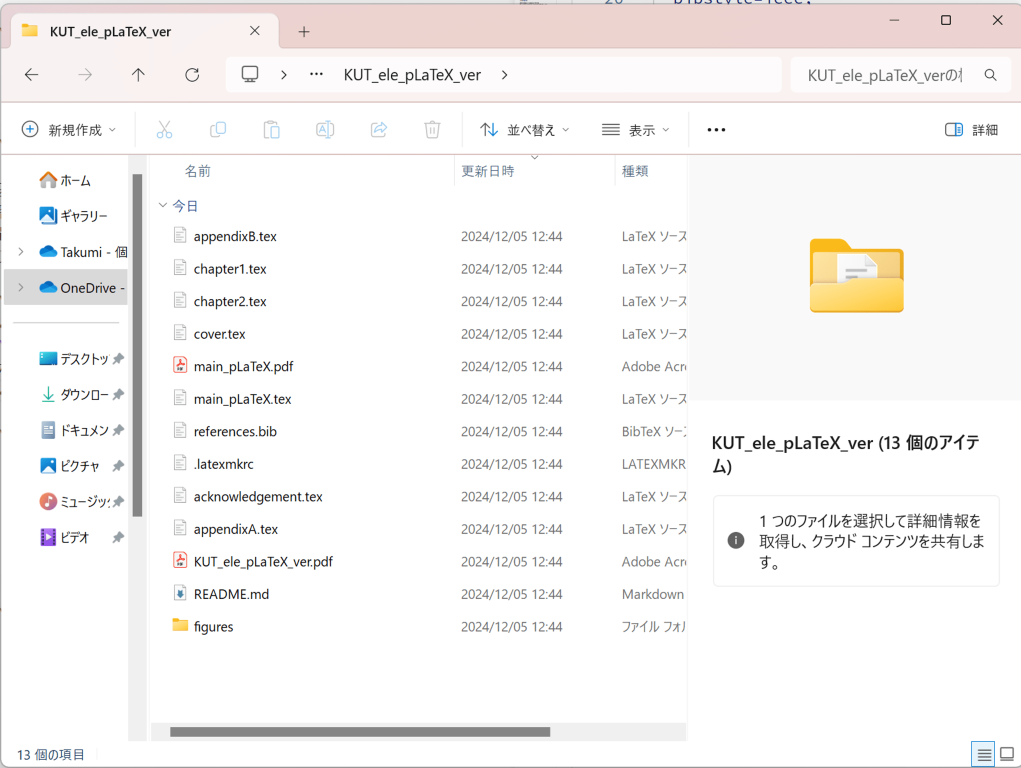
\includegraphics[keepaspectratio, width=0.8\linewidth]{open_code_from_current_directory.png}
  \caption{
    作業フォルダの一例.フォルダ上で右クリックして
    ここでは,KUT\_ele\_pLaTeX\_verというフォルダを作業フォルダとしている.
    一番下の項目「その他のオプションを確認」から「Codeで開く」を選択.}
  \label{fig:open code curr dir}
\end{figure}

\begin{figure}[tb]
  \centering
  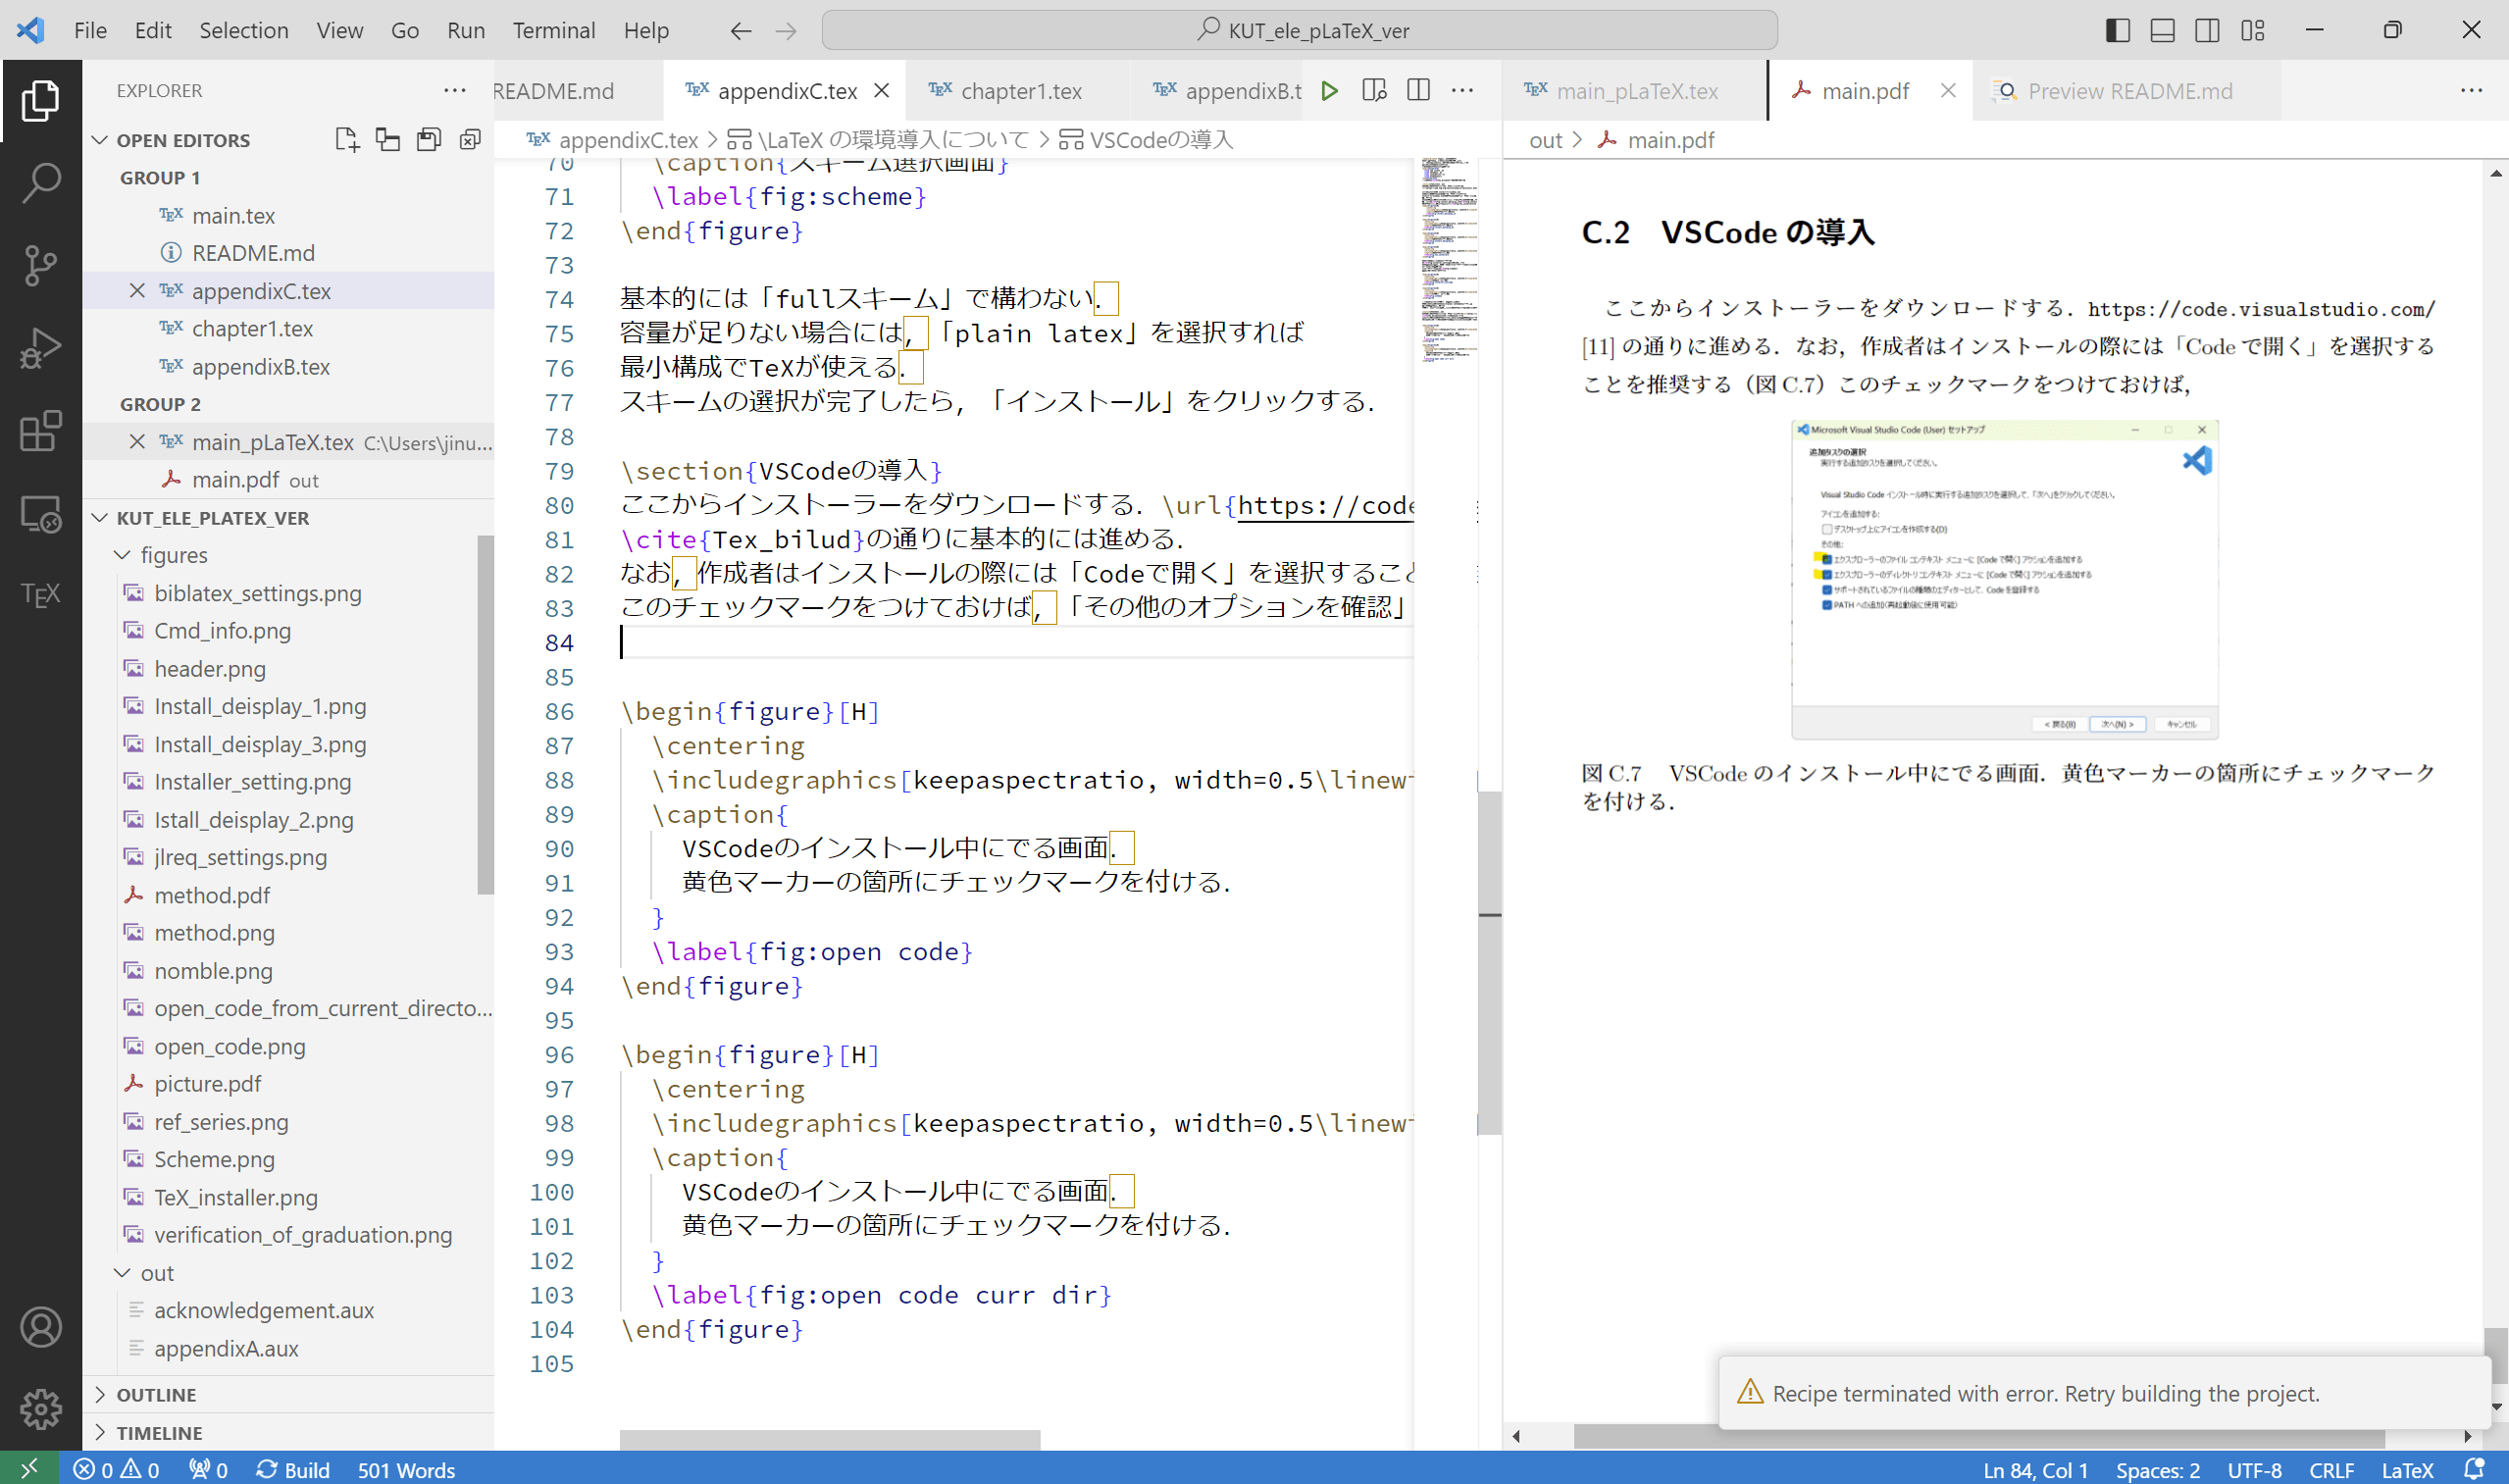
\includegraphics[keepaspectratio, width=0.8\linewidth]{open_work_dir.png}
  \caption{
    「Codeで開く」から開かれたVSCodeの一例.
    左側にKUT\_ELE\_PLATEX\_VERフォルダの中身の一覧が表示されている.
  }
  \label{fig:open work dir}
\end{figure}

\section{GitHubの活用}
Github\_settingフォルダがKUT\_ele\_LuaTeX\_verとKUT\_ele\_pLaTeX\_verと同じ階層に
あるので,フォルダ内のgithub.pdfを参照すること.


% ========================= 本文終了 =================================== %
% \printindex % 索引出力
\end{document}